\documentclass[12pt]{article}
\usepackage{mathtools,amssymb,graphicx}
\usepackage{fullpage}
\usepackage{parskip}
\usepackage{enumitem}
\usepackage{hyperref}

\pagestyle{empty}

\newcommand{\sol}{\textbf{\textit{Solution: }}}
\newcommand{\solnum}[1]{\textbf{\textit{Solution #1: }}}

\begin{document}
\begin{center} \bfseries \large
    January Monthly Problem Set

    Due date: 17 January 2025
\end{center}

\bigskip
Submit your monthly problem sets here: \url{https://forms.gle/pZH93Fq95UuABT277}.
You can ask the coaches from the Stellenbosch Camp for hints, but do not ask other people for help or look for help online.

\begin{enumerate}[topsep=\bigskipamount,itemsep=\bigskipamount,leftmargin=0pt]
% G
\item % Stellenbosch Camp 2005
Let $\triangle{ABC}$ be right-angled at $C$ with $BC= CA$, and $D$ be a point on the line $BC$ beyond $C$ such that $CD < BC$.
Furthermore, let $E$ be on the segment $AC$ such that $CE=CD$ and let $P, Q, R, S$ be the midpoints of $AB, BD, DE, EA$ respectively.
Prove that $PQRS$ is a square.

\solnum{1}
$\triangle ACD$ and $\triangle ECB$ are congruent (SAS) and rotated by $90^\circ$,
hence $AD=EB$ and $AD\perp BE$.
In $\triangle ADB$, $P$ and $Q$ are the midpoints of $AB$ and $DC$ respectively,
hence by the midpoint theorem,
$PQ=AD/2$ and $PQ\parallel AD$.
Similarly for $SR$, $RQ$, $SQ$ in triangles
$AED$, $DEB$, $AEB$ respectively.
Thus $PQ=SR=AD/2=EB/2=SP=RQ$
and $PQ\parallel SR\parallel AD\perp EB\parallel SP\parallel RQ$.
Thus $PRQS$ is a square.

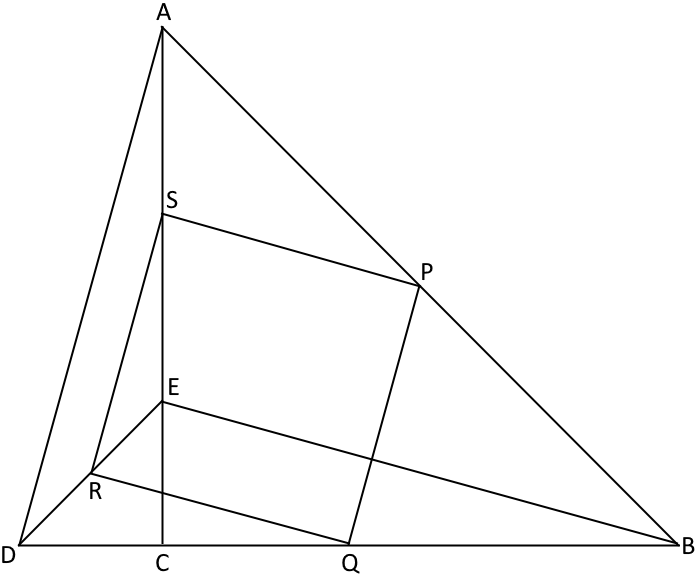
\includegraphics[scale=0.5]{Advanced/M1 Q1.png}

\solnum{2}
Without loss of generality let $CB = 2$ and $DC = 2x$.
Place the diagram in the complex plane 
with $C=0$, $B=2$ $A = 2i$, then, $D = -2x$, and $E=2xi$.
Then 
$$\begin{array}{r@{\,}l@{\,}l}
    P &= (A+B)/2 & = 1+i\\
    Q &= (B+D)/2 & = 1-x\\
    R &= (D+E)/2 & = -x+ix\\
    S &= (A+E)/2 & = xi+i\\
    P-Q & = x+i &\\
    Q-R & = 1-ix & = -i(P-Q)\\
    R-S & = -x-i & = -i(Q-R)
\end{array}$$
Thus $P-Q$, $Q-R$, and $R-S$ have the same length and are rotated by $90^\circ$ the same way.
Thus $PQRS$ is a square.

% AC
\item Find the number of tuples $(x_1, x_2, \dots, x_{50})$ of real numbers such that $x_1 = 2$, $x_2 = 3$, and for all $i\in \{1,2,\dots,50\}$, we have
$$(x_i+x_{i+1})^2 = (x_{i+1} + x_{i+2})^2,$$
where $x_{51} = x_{1}$ and $x_{52} = x_{2}$.

\sol
For each $i$, let $y_i = (-1)^i x_i$.
%This is a bijective mapping from $x_i$ to $y_i$
%for $1\leq i\leq 50$.
Conveniently $y_{51} = -x_{51} = -2 = -x_1 = y_1$
and $y_{52} = x_{52} = 3 = x_2 = y_2$.
%Hence this mapping applies for $i\in\{51,52\}$,
%with the restriction $y_{51} = y_1 = -2$ and %$y_{52} = y_2 = 3$.

Also $(x_i+x_{i+1})^2 = ((-1)^i y_i+(-1)^{i+1} y_{i+1})^2 = (-1)^{2i}(y_i-y_{i+1})^2$.
Thus 
\begin{align*}
    (y_i - y_{i+1})^2 & = (y_{i+1}-y_{i+2})^2\\
    |y_i - y_{i+1}| & = |y_{i+1}-y_{i+2}|\\
    |y_{i+1} - y_i| & = |y_2 - y_1| = 5\\
    y_{i+1} = y_i + 5 & \text{ or } y_{i+1} = y_i - 5
\end{align*}

For each $i\in\{1,\dots,51\}$, let $t_i = (y_{i+1}-y_i)/5\in\{-1,1\}$,
thus 
\begin{align}
y_{i+1} & = y_1 + 5(t_1 + \dots + t_{i}) \label{qu2_10}\\
y_1 & = y_{51} = y_1 + 5(t_1 + \dots + t_{50})\nonumber\\
0 & = t_1 + \dots + t_{50}\label{qu2_12}\\
y_{52}-y_{51} & = y_2-y_1 = 5\nonumber\\
t_{51} & = t_1 = 1\label{qu2_15}
\end{align}
But each $t_i\in\{-1,1\}$, thus by (\ref{qu2_12}) the tuple $(t_1, \dots, t_{50})$ will contain twenty five $1$'s and twenty five $-1$'s with $t_1$ being fixed to $1$.
%Thus from $y_1$ to $y_{i+1}$ there will be several $5$'s added and subtracted from $y_1$,
%total number of $5$'s being $i$.
%But $y_{51} = y_1$,
%thus the number of $5$'s added must balance the number of $5$'s subtracted,
%with fifty $5$'s in total.
%Hence there are twenty five $5$'s added and twenty five $5$'s subtracted.
There are $\binom{49}{24}$ ways to rearrange the last $1$'s and $-1$'s, hence there are at most $\binom{49}{24}$ of the original tuples.

Conversely, each of these rearrangements of $1$'s and $-1$'s with $y_1 = -2$, $(\ref{qu2_10})$, $(\ref{qu2_12})$, $(\ref{qu2_15})$ and $x_i = (-1)^i y_i$ give values of $x_i$ which satisfy the given.

Because
\begin{align*}
  \forall i\in\{1,\dots, 52\} &&  x_i & = \left(-2 + 5\sum_{j=1}^{i-1} t_i\right)(-1)^i\\
  \forall i\in\{1,\dots, 51\} &&  x_i + x_{i+1} & = \left(\left(-2 + 5\sum_{j=1}^{i-1} t_i\right)-\left(-2 + 5\sum_{j=1}^{i} t_i\right)\right)(-1)^i\\
  &&& = 5t_i(-1)^i\\
  \forall i\in\{1,\dots, 51\} &&  (x_i + x_{i+1})^2 &  = 25\\
  \forall i\in\{1,\dots, 50\} &&  (x_i + x_{i+1})^2 &  = (x_{i+1} + x_{i+2})^2\\
  && x_1 & = -y_1 = 2\\ 
  && x_2 & = y_2 = -2 + 5t_1 = 3\\
  && x_{51} & = -y_{51} = -(-2 + 5(t_1 + \dots + t_{50})) = -(-2) = x_1\\
  && x_{52} & = y_{52} = -2 + 5(t_1 + \dots + t_{50} + t_{51}) = -2 + 5t_{51} = 3 = x_2
\end{align*}

\textbf{\textit{Marking Scheme:}}
\begin{itemize}
    \item Basic ideas 2 marks max
    \begin{itemize}
        \item Observe $|x_i + x_{i+1}| = 5$.
        \item Observe we two choices for each $x_{i+1}$ given $x_i$ independently but not every one of these choices is valid.
        \item Find two solutions.
    \end{itemize}
    \item Deduce that there are at most $\binom{49}{24}$ solutions. 3 marks
    \begin{itemize}
        \item Method 1: Observe a grid pattern. 1 mark.
        Show that two different routes go to back to the same value. 2 marks
    \end{itemize}
    \item Write down the answer of $\binom{49}{24}$. 1 mark
    \item Show that every one of the ways claimed to work actually work
    (many students would have discovered that their claimed number was just an upper bound if they did this step). 
    This is the same as showing that you fully used every bit of given information. 1 mark
\end{itemize}
% A
\item Let \(r\), \(s\), and \(t\) be positive real numbers. Show that
\[r^{2} + s^{2} + t^{2} + 2rst + 1 \geqslant 2(rs + st + tr).\]

\solnum{1}
It is sufficient to prove this for $r$ a non-negative real number and I will do so.

\textit{Case} $0 \leqslant r \leqslant 2$:
\begin{align*}
    && r^{2} + s^{2} + t^{2} + 2rst + 1 & \geqslant 2(rs + st + tr)\\
    \iff &&  (r-1)^2+ 2r + s^2 + t^2 + 2rst & \geqslant 2(rs + st + tr)\\
    \impliedby && 2r + s^2 + t^2 + 2rst & \geqslant 2(rs + st + tr)
\end{align*}

The left hand side minus the right hand side
is linear in $r$.
A linear function achieves its minimum on
at least one of its endpoints.
Hence if this failed,
then it would fail on at least one at its endpoints.
Hence it is sufficient to check
that it holds at the endpoints $r=0$ and $r=2$.

\textit{Subcase} $r=0$: $s^2 + t^2\geqslant 2st$ which is always true.

\textit{Subcase} $r=2$:
\begin{align*}
    && 4 + s^2 + t^2 + 4st & \geqslant 2(2s + st + 2t)\\
    \iff && (s+t-2)^2 & \geqslant 0
\end{align*}
which is always true.

\textit{Case} $r \geqslant 2$:
\begin{align*}
    && r^{2} + s^{2} + t^{2} + 2rst + 1 & \geqslant 2(rs + st + tr)\\
    \impliedby && r^{2} + s^{2} + t^{2} + 4st + 1 & \geqslant 2(rs + st + tr)\\
    \iff && (r-s-t)^2 + 1 & \geqslant 0
\end{align*}
which is always true.

\solnum{2}
If $r \geqslant 2$, $s \geqslant 2$ or $t \geqslant 2$,
then this is identical to the first solution.
Assume $0 < r,s,t < 2$.
\begin{align*}
    && r^{2} + s^{2} + t^{2} + 2rst + 1 \geqslant 2(rs + st + tr)\\
    \iff && r^{2} + 2r(st-s-t) + (s^{2} + t^{2} -2st + 1) \geqslant 0
\end{align*}
This is a quadratic in $r$
with positive $r^2$ term.
This inequality will hold for all $r$
if the discriminant is always non-negative.
\begin{align*}
    \impliedby && 4(st-s-t)^2 - 4(s^{2} + t^{2} -2st + 1)  & \leqslant 0\\
    \iff && s(s-2)t(t-2) & \leqslant 1\\
    \iff && (1-(s-1)^2)(1-(t-1)^2)  & \leqslant 1
\end{align*}
But $0 < s < 2$,
thus $-1 < s-1 < 1$,
thus $0\leqslant (s-1)^2 < 1$,
thus $0 < 1-(s-1)^2 \leqslant 1$.
Similarly $0 < 1-(t-1)^2 \leqslant 1$.
Thus $(1-(s-1)^2)(1-(t-1)^2)  \leqslant 1$
as required.

\solnum{3}
Let \(x = r^{1/3}\), \(y = s^{1/3}\), and \(z = t^{1/3}\). We have
\begin{align*}
    &\mathrel{\phantom{=}} r^{2} + s^{2} + t^{2} + 2rst + 1 & & \\
    &= x^{6} + y^{6} + z^{6} + (x^{3}y^{3}z^{3} + x^{3}y^{3}z^{3} + 1) & & \\
    &\geqslant x^{6} + y^{6} + z^{6} + 3x^{2}y^{2}z^{2} & & \textrm{(AM-GM)}\\
    &\geqslant (x^{4}y^{2} + x^{2}y^{4}) + (y^{4}z^{2} + y^{2}z^{4}) + (x^{4}z^{2} + x^{2}z^{4}) & & \textrm{(Schur)}\\
    &\geqslant 2x^{3}y^{3} + 2y^{3}z^{3} + 2z^{3}x^{3} & & \textrm{(AM-GM)}\\
    &= 2(rs + st + tr).
\end{align*}

\solnum{4}
By AM-GM for \(rst\), \(rst\), and 1, we have
\begin{align*}
    &\phantom{=} r^{2} + s^{2} + t^{2} + 2rst + 1\\
    &\geqslant r^{2} + s^{2} + t^{2} + 3(rst)^{2/3}\\
    &\geqslant 2(rs + st + tr)
\end{align*}
by Popoviciu's inequality applied to the convex function \(\mathbb{R} \implies \mathbb{R}: x \mapsto e^{x}\) and the numbers \(2 \ln r\), \(2 \ln s\), and \(2 \ln t\).

% CG 
% Does not seem free ChatGPT-able nor googlable
\item 
How many ways are there to divide a regular pentagon into 5 triangles of equal area?

\solnum{1}
Let $ABCDE$ be the regular pentagon 
and let $F$ be its circumcenter.

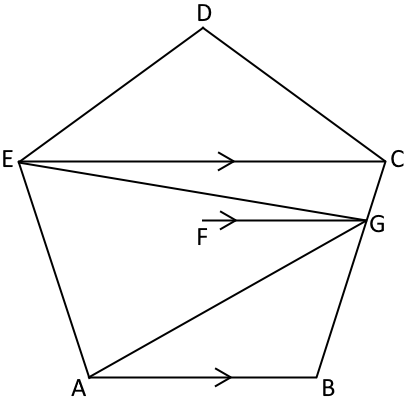
\includegraphics[scale=0.5]{Advanced/M1 Q4.png}

One obvious way to divide the pentagon
is to join its vertices to $F$
and form $5$ congruent triangles of equal area.
I will show that this is the only way.

Without loss of generality let the area of the pentagon be $5$.
Thus $|AFB| = 1$.

Every side must be covered by the five triangles.
Each triangle could cover no part of any side, part to all of one side, or part to all of two adjacent sides.

Assume for a contradiction that a triangle covers part to all of two adjacent sides.
Without loss of generality let those two sides be $AB$ and $BC$.

I will firstly show a cut that almost works.
Draw line $FG\parallel AB$ so that it cuts $BC$ at $G$.
Note $G$ will lie on the line segment $BC$ because $C$ lies above $F$ as measured from $AB$ because $C\hat{F}A + F\hat{A}B = 2(72^\circ) + 108^\circ/2>180^\circ$.

Draw triangles $ABG$, $EGC$, $EDC$ and any two triangles that equally divide $AEG$.

$|ABG| = |ABF| = 1$ because they have the same height.
\begin{align*}
    |EGC|+|EDC| &= |EFC|+|EDC| && \text{(same height)} \\
    &= |EFD|+|DFC| \\
    &= 2
\end{align*}
But $|EDC| = \frac{1}{2}ED\cdot DC\sin(108^\circ) > \frac{1}{2}AB\cdot BG\sin(108^\circ) = |ABG| = 1$,
thus $|EGC| < 1$.
Thus this cut does not work.

Now suppose that we pick another triangle $A'BG'$
containing part to all of $AB$ and $BC$;
with $A'$ on segment $AB$, 
and $G'$ on segment $BC$.
Without loss of generality assume $CG' \geq AA'$.

Now $\frac{1}{2} AB\cdot BG\sin(180^\circ) = |ABG| = 1 = |A'BG'| = \frac{1}{2} A'B\cdot BG'\sin(180^\circ)$.
Now because $A'B\leq AB$, thus $BG'\geq BG$, thus $CG'\leq CG$.
Also if $BG = BC$, then $A'B = BG$, but this contradicts $CG' \geq AA'$.
Thus $0 < CG'\leq CG$.

One of the triangle cuts, say $XYZ$, must cover part or all of $CG'$; without loss of generality let $XY$ lie on line segment $CG'$.
Hence $XY \leq CG'$.
And $XYZ$'s maximum possible height measured as from $BC$ would be the height of $EGC$.
Thus $|XYZ| \leq |EGC| < 1$.
Thus the cut will not be large enough, a contradiction.

Thus no triangle can cover more than one side, thus each triangle must cover at most one side.
Thus each triangle can cover at most the length of $AB$ of the perimeter, but all five triangles must cover five times the length of $AB$, thus every triangle must cover exactly one side.

Let $ABH$ be one such triangle, with $H$ strictly inside $ABCDE$.
Assume for a contradiction that $H\neq F$.

Another triangle must have $H$ as its vertex because: 
The area inside the reflexive angle $A\hat{H}B$ immediately around and up $H$ must be covered.
An edge of another triangle going through $H$ would remove exactly $180^\circ$
of this area.
Another triangle sharing a vertex with $H$ would remove smaller parts of this area.
Hence at most one edge of the other triangles can go through $H$, but reflective $A\hat{H}B>180^\circ$, meaning at least some of it must be covered
by a triangle having vertex $H$.
Let that triangle be $HXY$ where $XY$ is one of the sides of $ABCDE$.

Now $|HAB| = |FAB|$, hence $HF\parallel AB$ because $H\neq F$, similarly $HF\parallel UV$.
Thus $AB\parallel UV$, a contradiction.

Thus $H=F$. Apply this to all sides of $ABCDE$, showing all the triangles must have a side of $ABCDE$ and have $F$ as a vertex.
Hence this is only cut that works and the answer is 1.

\solnum{2}
Let $ABCDE$ be the regular pentagon and let $F$ be its circumcentre.

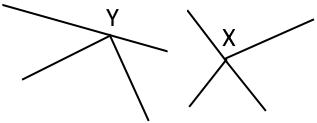
\includegraphics[scale=0.5]{Advanced/M1 Q4b.png}

There are three types of points where the triangle's vertices could be at.
Call a point an $X$ type point if it is not strictly inside any edge of any triangle or pentagon.
Call a point a $Y$ point if it is a vertex of a triangle and strictly inside an edge.
Call the original vertices of the pentagon as $Z$ points.

The sum of the angles from the triangles surrounding each $X$ point is $2\times 180^\circ$.
The sum for each $Y$ point is $180^\circ$ (counting only angles at a triangle's vertex).
The sum for all $Z$ points is $3\times 180^\circ$.
The sum of all the triangles' angles is $5\times 180^\circ$.
Hence there are either exactly two $Y$ points or one $X$ point.

If an edge of the pentagon is not subdivided by an $Y$ point, then that edge must be part of a triangle and the triangle's third vertex must be on a line parallel to the side going through $F$.
None of the $Z$ points lie on this line, hence the third point must be an $X$ or $Y$ point.

There are at most two $X$ or $Y$ points.
There are at least three sides of the original pentagon that are not subdivided.
Therefore by PHP two of these must share an $X$ or $Y$ point.
This point must lie on the lines through $F$ and parallel to those two sides,
hence it must be $F$.

Thus there are at least four sides not subdivided.
But only $F$ can be an $X$ or $Y$ point shared by the triangles containing these types of sides.
Thus at least three of them share $F$.
Each of them make an angle of $72^\circ$ at $F$, thus $F$ must be a $X$ point.

Thus there are no $Y$ points and thus all sides are not subdivided and their triangles must connect to the only $X$ point namely $F$.

\solnum{3}
An outline of a solution.

Let $O$ be the circumradius which is also the incenter.
Let $F$ be the point where the incircle touches $ED$ and by symmetry the midpoint of $ED$.
Let $J$ be on $OB$ such that $OF=OJ$.
Let $X$ lie on $AB$ and $Y$ on $BC$ such that $XY\parallel ED$ and $J$ lies on $XY$.

Let $x$ be the inradius of the incircle.
Let $T$ be the area of each triangle.

Thus $OE = x/\cos 36^\circ$ and $ED = 2EF = 2x \tan 36^\circ$
and $T = \frac{1}{2} OF\cdot ED = x^2 \tan 36^\circ$.

\textit{Lemma 1:}
$T < |EDA| < 2T$.

\textit{Proof lemma 1:}
Now $AC\parallel ED$, hence either $A$ and $C$ both lie above $O$ or below $O$
as measured from $ED$.
Thus $\angle AOC$ to the side of $ED$ is either reflexive or not reflexive respectively.
Now this $\angle AOC = 2\angle ABC = 216^\circ$.
Hence $A$ is above $O$,
hence $|AEB| > |OED| = T$.

Clearly $A$ lies below $X$.
[If it did not then, $X$ lies below $A$ on $AB$ extended through $A$ but besides being absurd in even a badly drawn diagram, this would also contradict lemma 2].
Thus $|AED| < |EDX| = |EJD| = 2T$.\text{End proof of Lemma 1}

\textit{Lemma 2}
Any triangle $M_1 M_2 M_3$ inside the pentagon with $M_1 M_2 \leq BX$ will have $|M_1 M_2 M_3| < T$.

\textit{Proof Lemma 2:}
The largest possible length of $M_1 M_3$ would be the furtherest distance between two points of the pentagon, which is $AD$.
(For any polygon, the distance between any two of its points will be less than equal to furthest distance between two of its vertices).

Now
\begin{align*}
    AD &= \dfrac{ED \sin \angle AED}{\sin \angle EDA}
    = \dfrac{2x \tan 36^\circ \sin 108^\circ}{\sin (180^\circ-\angle AED/2)} \\
    &= \dfrac{2x (\sin 36^\circ/\cos 36^\circ) \sin 72^\circ}{\sin 36^\circ}
    = \dfrac{2x \sin 72^\circ}{\cos 36^\circ}
    = 4x \sin 36^\circ.
\end{align*}
\begin{align*}
    \text{Now } BJ &= OB - OF = OE - OF = x(-1+1/\cos 36^\circ) \\
    XB &= BJ/\sin 36^\circ = x(-1+1/\cos 36^\circ)/\sin 36^\circ = \dfrac{x(1-\cos 36^\circ)}{\cos 36^\circ \sin 36^\circ}
\end{align*}
\begin{align*}
    |M_1 M_2 M_3| &= \frac{1}{2} M_1 M_2 \cdot M_1 M_3
    \leq \frac{1}{2} (4x \sin 36^\circ) \left(\dfrac{x(1-\cos 36^\circ)}{\cos 36^\circ \sin 36^\circ}\right) = \dfrac{2x^2 (1-\cos 36^0)}{\cos 36^\circ}
\end{align*}
\begin{align*}
    |M_1 M_2 M_3| &< T \\
    \impliedby \dfrac{2x^2 (1-\cos 36^0)}{\cos 36^\circ} &< x^2 \tan 36^\circ
    & \impliedby 2 (1-\cos 36^0) &< \sin 36^\circ \\
    \impliedby 4(1-\cos 36^\circ + \cos^2 36^\circ) &< \sin^2 36^\circ &\text{(both sides are positive)} \\
    \impliedby 3-4\cos 36^\circ + 5\cos^2 36^\circ &< 0 \\
    \impliedby (1-\cos 36^\circ)(3-5\cos 36^\circ) &< 0 \\
    \impliedby 3-5\cos 36^\circ &< 0 &\text{because } 1-\cos 36^\circ &> 0 \\
    \impliedby \frac{3}{5} &< \cos 36^\circ
    & \impliedby \frac{3}{5} < \sqrt{0.5} < \cos(45^\circ) &< \cos 36^\circ
\end{align*}
\textit{End proof Lemma 2}

Suppose that one of the sides of the pentagon contains 1 or more vertices of the triangles in its interior.
Without loss of generality let this side be $ED$,
Let these vertices be $K_1$, $K_2$, $\dots$, $K_n$ in that order from $E$ to $D$
Now $EK_1 \leq \frac{1}{2}ED$ or $K_n D\leq \frac{1}{2} ED$.
Without loss of generality let $EK_1 \leq \frac{1}{2}ED$.
Rename $K_1$ to $G$.

Let $R$ be the third point of the triangle with side $EG$.
Now
\begin{align*}
    &\mathrel{\phantom{\implies}} |EGR| = |EOD| \\
    &\implies \text{`height with respect to EG'}\cdot EG = OF\cdot ED \\
    &\implies \text{`height with respect to EG'}\geq 2 OF
\end{align*}
Thus $R$ is on or above $XY$ (with respect to $EG$).

Case $R=B$: Thus $EB$ splits $ABE$ off,
hence an integer number of triangles must fit in $ABE$ exactly.
But by lemma 1, this is impossible.

Case $R$ is on segments $BX$ or $BY$:
There must be triangle(s) that covers $RB$,
hence they have a side less than $RB \leq BX$.
Hence by Lemma 2, their area cannot be sufficiently large.

Case $R$ lies inside $\triangle BYX$ excluding on $BX$, $BY$ or at $B$:
%Case $R$ lies below $B$:
The area above $R$ must be covered
%the reflexive $\angle ERG$ must be covered
by other triangles.
Let $N_1 N_2 N_3$ be one such a triangle.
Without loss of generality let $l=N_1 N_2$ be a line segment containing $R$ (possibly at its endpoints)
with $N_1$ at least above $N_2$ with respect to $ED$.
%and $l$ is side of a triangle which covers the area above $R$ with its own points near $l$.

Subcase $l \parallel  XY$:
then $N_1 N_2 N_3$ will be contained within $BXY$ and hence by lemma 2 its area would be too small.

Subcase $l \not\parallel  XY$:
If $N_1 = R$,
then the only way for $N_1 N_2 N_3$ to cover the area above $R$ is for $N_3$ to be above $R$,
but then we could have defined $N_2 N_3$ as $l$,
so without loss of generality assume $N_1$ is above $R$.

If $N_2$ is below $R$, then $N_3$ must be on the opposite side of $l$ as $E$ and $G$ to avoid overlapping.
The $180^\circ$ angle $\angle N_1 R N_2$ on the opposite side of $l$ as $N_1$
is partially covered by $\angle ERG$,
so the angle $\angle N_2 R G$ or $\angle N_2 R E$
must be covered,
specifically the part of this angle closest $N_2 R$,
but this will create a triangle a side on $R$ and $R$ as the lowest point of this side.
Hence without loss of generality assume $N_2 = R$.

Another way to reason through these cases: 
The angle around $R$ must be covered, it can either be covered by a side of a triangle making a $180^\circ$ at $R$ and the rest of the angles being smaller than $180^\circ$ thus vertices of the triangles and thus line segments starting at $R$,
or it can be covered by only line segments starting at $R$.
In either cases consider a line $X'Y'\parallel XY$
and the line segments above this line
(unless they are parallel to this line).

Rename $N_1$ as $R_2$.
Like $R$ there are three cases for where $R_2$ is.
Similarly if $R_2\neq B$, then this will lead to contradiction or point $R_3$,
we cannot produce points like this indefinitely because there are finite number of triangles.
If $R_2 = B$, 
then $R R_2$ (which is $N_2 N_1$)
will be shorter than $BX$ which is a contradiction by lemma 2.

Thus in these cases, there cannot be more than one point on a side.

By similar logic to proof one, the proof can be completed.

Marking scheme
\begin{itemize}
\item Proof of lemma 1. 1 mark
\item Proof of lemma 2. 2 marks
\item List all possible positions for for $R$ and $R_2$. 1 mark
\item Noticing $R_2$ is similar to $R$. 1 mark
\item Reason through all cases of another side going through $R$. 1 mark
\item Case where there are no points on the triangle sides. 
(One the one hand, this is a smaller percentage of work compared to the other solutions.
But it is not absolutely less work. 
However a half of the work overlaps with properly reasoning about what happens around $R$).
1 mark
\end{itemize}

\solnum{4}
Similar to solution 3 but a bit more combinatorial like solution 2.
In solution 2 we noted that there are three types of graphical vertices where the triangles vertices meet,
I called these $X$, $Y$ and $Z$ type vertices.
If a polygon is concave, then there can be a fourth type of point 
where a side of the triangle goes through a concave vertex.
Which I will call a $C$ type point.

Construct all points with the same names as solution 3, except don't draw $X$ and $Y$ as they are not needed.

Here are three lemmas that are very similar to those found in solution 1, 2 and 3.

\textit{Lemma 1:}
$T < |EDA| < 2T$.
%As a collary if $AD$ is a side of a triangle,
%then its third vertex will be below $BC$.

\textit{Lemma 2:}
If there are triangles that each have a different side of the pentagon as one of their sides
and they share their third point,
then that third point must be $O$.

\textit{Lemma 3:}
If there are $x$, $y$, $z$ and $c$ 
of $X$, $Y$, $Z$ and $C$ type vertices
in the graph created by $t$ triangles 
covering a concave polygon with $m$ non-reflexive vertices and $n$ reflexive vertices, then
\begin{align*}
    180t + 180c &= 180(m+n-2) + 360x + 180y \\
    z &\leq m+n \\
    c &\leq n \\
    z+c &= m+n
\end{align*}
Suppose that one of the sides of the pentagon contains 1 or more vertices of the triangles in its interior.
Without loss of generality similar to solution 3 we can construct a triangle $EGR$
with $G$ on $ED$, $EG \leq \dfrac{1}{2} ED$,
and $R$ above line $AC$ by lemma 1.

Case $R=B$: Thus $EB$ splits $ABE$ off,
hence an integer number of triangles must fit in $ABE$ exactly.
But by lemma 1, this is impossible.

Case $R$ is on segements $BA$:
This leaves convex $ERA$ and $DGRBC$ to cover with four triangles.
By lemma 3, $DGRBC$ will need $3$ triangles
and $ERA$ just one.
Thus $DC$ will be an uncut edge of some triangle,
by lemma 1 its  third vertex cannot be $G$ or $B$, so it must be $R$.
But $R$ is the third vertex of $ERA$ which contradictics Lemma 2.

Case $R$ lies on $BC$:
This leaves convex $ERBA$ and $DGRC$.
Now $AB$ needs a third vertex, it cannot be $E$ by lemma 1 and it cannot be $R$ because this would be third vertex of $EA$ too contradicting lemma 2.

Case $R$ lies inside $\triangle ABC$ excluding on $BA$, $BC$ or at $B$:
This would leave a septagon with one reflex angle,
thus by lemma 3, there are no $X$ or $Y$ type vertices.
Now $AB$ needs a third vertex,
this can only be $R$ by lemma 1.
Similarly for $BC$,
but then $R$ is shared by these sides,
but $R\neq O$ a contradiction.





By using similar logic to proof 1, the proof can be completed.

Marking scheme
\begin{itemize}
\item Proof of lemma 1. 1 mark
\item Proof of lemma 2. 1 mark
\item Proof of lemma 3. 2 marks
\item Work through all possible positions for $R$. 2 marks
\item Case where there are no points on the triangle sides. 1 mark
\end{itemize}

% A
\item Let $f: \mathbb{N}_0 \implies \mathbb{R}$ be a function with $f(0) = 0$ such that for all $n \in \mathbb{N}_0$ we have
$$n \leqslant f(n) + f(n+1) \leqslant 2n.$$
\begin{enumerate}[itemsep=0pt]
    \item Show that for all $n \geqslant 2$, we have
    $$|f(2n)| + |f(2n+1)| \leqslant 2n^2.$$
    \item Find all such $f$ such that, for all $n \in \mathbb{N}_{0}$, we have $$|f(2n)| + |f(2n+1)| = 2n^2.$$
\end{enumerate}

\sol
Let $g(n) = (-1)^n f(n)$.
Thus $g(0) = f(0) = 0$
Our condition becomes
$$\begin{array}{r@{\,}c@{\,}l}
  n\leq & g(n)(-1)^n + g(n+1)(-1)^{n+1} & \leq 2n \\
  -n/2\leq & g(n)(-1)^n + g(n+1)(-1)^{n+1} -3n/2 & \leq n/2 \\
  -n/2\leq & g(n+1) - g(n) -3n(-1)^{n+1}/2 & \leq n/2
\end{array}$$
Adding these inequalities
from $n=0$ to $n=m-1$
we get
$$\begin{array}{r@{\,}c@{\,}l}
\dfrac{-m(m-1)}{4}\leq & g(m) + {\displaystyle\frac{3}{2}\sum_{n=0}^{m-1}} (-1)^n n & \leq \dfrac{m(m-1)}{4}\\
\dfrac{-m(m-1)}{4}\leq & g(m) + \dfrac{3}{2}\left\lceil\dfrac{m-1}{2}\right\rceil(-1)^{m-1} & \leq \dfrac{m(m-1)}{4}\\
\dfrac{-m(2m-1)}{2}\leq & g(2m) - \dfrac{3m}{2} & \leq \dfrac{m(2m-1)}{2}\\
\dfrac{-2m^2+4m}{2}\leq & g(2m)& \leq \dfrac{2m^2+2m}{2}\\
\dfrac{-m(2m+1)}{2}\leq & g(2m+1) + \dfrac{3m}{2} & \leq \dfrac{m(2m+1)}{2}\\
\dfrac{-2m^2-4m}{2}\leq & g(2m+1)& \leq \dfrac{2m^2-2m}{2}\\
-2m^2 \leq & g(2m) + g(2m+1) & \leq 2m^2
\end{array}$$
with equality on the left hand side if and only if every added inequality has equality on the left hand side.
Same for the right hand side.

Also from the original
$$\begin{array}{r@{\,}c@{\,}l}
  |f(2m+1) + f(2m)| & \leq 2m\\
  |g(2m+1) - g(2m)| & \leq 2m
\end{array}$$

Now 
$$\begin{array}{r@{\,}l}
  |f(2n)|+|f(2n+1)| & = |g(2n)|+|g(2n+1)|\\
  & =\begin{cases}
    |g(2n)+g(2n+1)| & \text{ if } g(2n)g(2n+1) > 0\\
    |g(2n)-g(2n+1)| & \text{ if } g(2n)g(2n+1) \leq 0
  \end{cases}\\
  & \leq \begin{cases}
    2n^2 & \text{ if } g(2n)g(2n+1) > 0\\
    2n & \text{ if } g(2n)g(2n+1) \leq 0
  \end{cases}\\
  & \leq 2n^2
\end{array}$$
With equality for $n\geq 2$ if and only if $g(2n)+g(2n+1)=\pm 2n^2$ and $g(2n)g(2n+1) > 0$.

If $g(2n)+g(2n+1)=2n^2$ for all $n\geq 2$,
then
all sums that produced $g(2n)+g(2n+1)=2n^2$
were equalities on the right hand side,
and those same equalities could be added to give
$g(2n)+g(2n+1)=2n^2$ for all $n\geq 0$.
The converse is trivial.

For all $n\geq 0$, 
$g(2n)+g(2n+1)=2n^2$ 
if and only if 
$g(2n) = n^2+n$ and $g(2n+1) = n^2-n$
if and only if
$f(2n) = n^2+n$ and $f(2n+1) = n-n^2$.
This is easily checkable to work.

Similarly for all $n\geq 2$, 
$g(2n)+g(2n+1)=-2n^2$ 
if and only if 
for all $n\geq 0$
$f(2n) = -n^2+2n$ and $f(2n+1) = 2n+n^2$.
This is easily checkable, but doesn't work since for $n=1$, we have $2n > n^2$, resulting in $|f(2n)| + |f(2n+1)| = 4n \neq 2n^2$.


% G
\item %Kazakhstan MO, 2008%
Inside a convex quadrilateral $ABCD$, let $P$ be a point such that $\angle APB=\angle ADP+\angle BCP$ and $\angle APD=\angle ABP+\angle DCP$.
Prove that $$AP\cdot CP+BP\cdot DP \geqslant \sqrt{AB\cdot BC\cdot CD\cdot DA}.$$

\solnum{1}
Do an inversion through $P$,
with points $A'$, $B'$, $C'$ and $D'$
the outputs of $A$, $B$, $C$ and $D$ respectively.

Draw line $PQ$ equal to $C'B'$
which splits $\angle APB$ 
into $\angle BPQ = \angle BCP$ 
and $\angle QPA = \angle ADP$.
Now $\angle BCP = \angle C'B'P$ from the inversion.
Thus $C'B'\parallel PQ$.
Similarly $D'A'\parallel PQ$.
Thus $C'B' \parallel D'A'$.
Similarly $\angle APD=\angle ABP+\angle DCP$
implies $C'D'\parallel B'A'$.
Thus $A'B'C'D'$ is a parallelogram.

$PQ = C'B' = D'A'$ and these are parallel,
hence $C'B'QP$ and $D'A'QP$ are parallelograms.

\begin{center}
    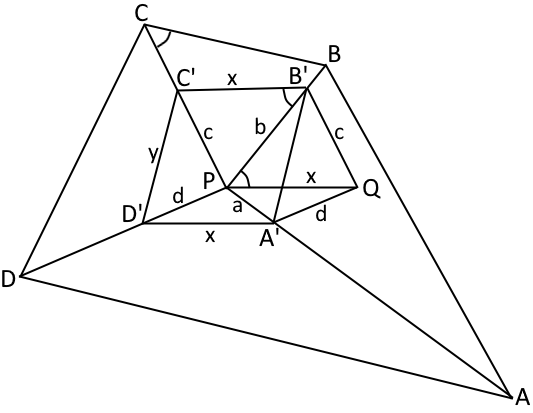
\includegraphics[width=0.6\textwidth]{Advanced/M1 Q6.png}
\end{center}

Let $PA'=a$, $PB'=b$, $PC'=B'Q=c$, $PD'=A'Q=d$,
$C'B'=PQ=A'D'=x$ and $C'D' = A'B'=x$.
Now by the inversion,
\begin{align*}
    && AP\cdot CP+BP\cdot DP & \geqslant \sqrt{AB\cdot BC\cdot CD\cdot DA}\\
    \iff && \dfrac{1}{a}\cdot \dfrac{1}{c}+\dfrac{1}{b}\cdot \dfrac{1}{d} & \geqslant \sqrt{\dfrac{y}{ba}\cdot \dfrac{x}{bc}\cdot \dfrac{y}{cd}\cdot \dfrac{x}{da}}\\
    \iff && bd+ac & \geqslant xy
\end{align*}
Which is Ptolemy in $PB'QA'$.

\solnum{2}\null
[Here are two theorems that I use all the time, but cannot find formal names for, hence I will prove them.]

\textbf{Sine ratio theorem}
If $0^\circ<\alpha,\beta,\theta,\phi,\alpha+\beta,\theta+\phi<180^\circ$,
$$\alpha+\beta = \theta+\phi \quad\text{and}\quad \dfrac{\sin \alpha}{\sin \beta} = \dfrac{\sin \theta}{\sin \phi}
\implies \alpha=\theta \quad\text{and}\quad \beta=\phi$$

\textbf{THEOREM PROOF}
Draw any triangle $ABC$ with $\angle A=\alpha$ and $\angle B = \beta$, this is possible because $0^\circ<\alpha,\beta,\alpha+\beta<180^\circ$.
Draw any triangle $XYZ$ with $\angle X=\theta$ and $\angle Z = \phi$.
Clearly 
$$\angle C = 180^\circ-\alpha-\beta=180^\circ-\theta-\phi = \angle Z$$
$$\dfrac{CB}{CA} = \dfrac{\sin\alpha}{\sin\beta}=\dfrac{\sin \theta}{\sin \phi}=\dfrac{ZY}{ZX}$$
$$\dfrac{CB}{ZY} =\dfrac{CA}{ZX}$$
Thus the triangles are similar,
thus $\alpha=\theta \text{ and } \beta=\phi$ \\
\textbf{END THEOREM PROOF}

\textbf{Generalized Ceva's Sine theorem}
For any point $P$ and polygon $A_1 A_2 \dots A_n$ with $n\geq 3$ and none of the sines below equal to zero, let $A_{n+1} = A_n$, then
$$\prod_{i=1}^n \dfrac{\sin \angle A_{i}A_{i+1}P}{\sin \angle A_{i+1}A_{i}P} = 1.$$
\textbf{THEOREM PROOF}
By the sine rule in each triangle $A_iA_{i+1}P$,
$$\prod_{i=1}^n \dfrac{\sin \angle A_{i}A_{i+1}P}{\sin \angle A_{i+1}A_{i}P}
=\prod_{i=1}^n \dfrac{A_{i}P}{ A_{i+1}P} =1$$
\textbf{END THEOREM PROOF}

[Warning, this theorem does not generalize the converse of Ceva's Sine Theorem.]

Draw line $RPQ$ which splits $\angle APB$ into $\angle BPQ = \angle BCP$ and $\angle QPA = \angle ADP$.
Thus $RPQ$ is tangent to circles $PCB$ and $PDA$, thus $\angle CPR = \angle CBP$ and $\angle RPB = \angle DAP$.
Thus $\angle CPD = \angle CBP + \angle DAP$.

Similarly $\angle APD=\angle ABP+\angle DCP$
implies $\angle BPC=\angle PDC+\angle PBA$.

[Now moving the various triangle around makes it seem quite plausible 
%that you can take $\triangle CPD$ rescale it and move it so that $C$ moves to $B$
moving and rescaling $\triangle CPD$ to fit next to $\triangle BPA$ will give a similar quadrilateral to the one created with $\triangle CBP$ and $\triangle DAP$.
Here is the proof of that.]

Draw line $PS$ to split $\angle APB$ as $\angle SPA = \angle BCP$ 
and $\angle BPS = \angle ADP$.
Choose the length of $PS$ such that $BPS ||| PDA$ and hence $\angle ABS = \angle DCP$.

Now compare the sum of angles in $APBS$ to $ABCD$ to get $0 < \angle ASP+\angle BAS=\angle PBC+\angle CDP < 180^\circ$.
Also compare the generalized Ceva sine rule to get $\dfrac{\sin \angle ASP}{\sin \angle BAS}=\dfrac{\sin\angle PBC}{\sin\angle CDP}$.
Thus by the `Sine ratio theorem', $\angle ASP=\angle PBC$ and $\angle BAS=\angle CDP$.

There are many similar triangles between $SBPA$ and $ABCDP$.
Express all lengths from
$AP\cdot CP+BP\cdot DP \geqslant \sqrt{AB\cdot BC\cdot CD\cdot DA}$
in terms of lengths in terms of $SBPA$,
this become Ptolemy in $SBPA$.

[Now it is possible to draw the original diagram by first drawing any $SBPA$,
thus we do not lose any generality by expressing everything in terms of the lengths of $SBPA$.
This is a heuristic of why this became a simpler problem.]
%C
%Does not seem free ChatGPT-able nor googlable
%You and six of your mathematician friends
\item
Jon Kariv is playing a game with six friends. Each of the seven people has a coloured sticky note placed on their back. Each of them can see the sticky note on everyone else but cannot see their own. There were two more sticky notes but they were hidden and no one was told their colours. In total there were three red, three yellow, and three green sticky notes, and everyone knows this. Jon's friends state the following statements one after another.
\begin{itemize}
\item First: ``I don't know the colour of my sticky note.''
\item Second: ``I also don't know my sticky note's colour.''
\item Third: ``I also don't know my sticky note's colour.''
\item Fourth: ``I have deduced that mine is red.''
\item Fifth: ``I have yet to deduce what the colour of mine is.''
\item Sixth: ``I have deduced that my sticky note is yellow.''
\end{itemize}
None of them are colour blind and are all perfectly logical.
Can you determine what colour Jon's sticky note is?

\sol
Let $K$ be the sentence
`I do not know my sticky notes colour'.
Let $A_1$, $A_2$, \dots, be those who say $K$ in order.
Let $F_n$ be 
the sticky notes of those who have not said $K$ 
after $A_n$ says $K$.

Observe the following invariant,
if $A_n$ says $K$, 
then there must be at least one of each colour in $F_n$.

Proof of this by induction,
when $A_1$ says $K$,
if the six other friends have at most two colours,
then the three other sticky notes,
including $A_1$'s note and the hidden notes,
must be of the remaining colour;
therefore $A_1$ could have deduced his colour,
a contradiction.

Assume this is true up to $A_n$ saying $K$,
thus there must be three colours amongst $F_n$.
Now $A_{n+1}\in F_n$.
If there are only two colours amongst 
$F_{n+1} = F_n-\{A_{n+1}\}$,
then $A_{n+1}$ would have had the third colour,
hence $A_{n+1}$ could deduce his colour,
a contradiction.
Thus the invariant holds by induction.

Thus when the fifth friend ($A_4$) says $K$,
there must be one of each colour with the fourth, sixth and seventh friends.

Thus Jon Kariv's colour is green.

% N
\item % Vietnam MO 1992
Let $n$ be a positive integer.
Let $f(n)$ be the number of divisors of $n$ that end with the digit 1 or 9, and let $g(n)$ be the number of divisors of $n$ that end with the digit 3 or 7.
Prove that $f(n) \geqslant g(n)$.

\solnum{1}
Let $u(n)$ be the number of distinct prime divisors in $n$.
Let $S(m)$ be the statement $f(n)\geq g(n)$ if $u(n) = m$.

Induction proof of $S(m)$.
Base cases $m = 1$, $m=0$:
Here is a table of $f(n)$ if $u(n)\leq 1$
$$\begin{array}{l|c|c}
    n & f(n) & g(n)\\ \hline
    1 & 1 & 0\\
    p^t \text{ where } p\equiv_{10} \pm 1 & t+1 & 0\\
    p^t \text{ where } p\equiv_{10} \pm 3 & \left\lceil \dfrac{t+1}{2} \right\rceil & \left\lfloor \dfrac{t+1}{2} \right\rfloor\\
    2^t  & 1 & 0\\
    5^t  & 1 & 0\\
\end{array}$$
Hence $S(0)$ and $S(1)$.

Induction step: for an arbitrary $i\geq 1$, assume $S(i)$.
For any $n$ with $u(n) = i+1$, there exists $n_1$, $n_2$ with $n=n_1 n_2$ and $\gcd(n_1, n_2) = 1$ and $u(n_1)= i$ and $u(n_2)= 1$.
Now $k\mid n_1 n_2$ if and only if there exists unique integers $k_1\mid n_1$ and $k_2\mid n_2$ such that $k = k_1 k_2$.

$k = k_1 k_2\equiv_{10} \pm 1$ if and only if ($k_1\equiv_{10} \pm 1$ and $k_2\equiv_{10} \pm 1$) xor ($k_1\equiv_{10} \pm 3$ and $k_2\equiv_{10} \pm 3$).
Therefore $f(n_1 n_2) = f(n_1) f(n_2) + g(n_1) g(n_2)$.

$k = k_1 k_2\equiv_{10} \pm 3$ if and only if ($k_1\equiv_{10} \pm 1$ and $k_2\equiv_{10} \pm 3$) xor ($k_1\equiv_{10} \pm 3$ and $k_2\equiv_{10} \pm 1$).
Therefore $g(n_1 n_2) = f(n_1) g(n_2) + g(n_1) f(n_2)$.

But $f(n_1) \geq g(n_1)$ and $f(n_2) \geq g(n_2)$,
therefore by the Rearrangment Inequality 
$$f(n_1 n_2) = f(n_1) f(n_2) + g(n_1) g(n_2) \geq f(n_1) g(n_2) + g(n_1) f(n_2) = g(n_1 n_2)$$

\textit{\textbf{Marking scheme:}}
\begin{itemize}
    \item Observe without loss of generality $2\nmid n$ and $5\nmid n$.
    (implicitly done in this proof) 1 mark
    \item Case $n=1$ within an induction argument. 1 mark
    \item Case $n=p^k$ (often implicitly in students proofs). 1 mark
    \item reason about what happens if you multiply a set of divisors by a prime ending in a certain digit. 1 mark
    \item Show $f(n_1 n_2) = f(n_1) f(n_2) + g(n_1) g(n_2)$
    and similar (often implicitly). 1 mark
    \item rearrangement inequality or similar. 1 mark
    \item Use necessary one to one mappings, and/or if and only if statements and/or obvious partitions of the divisors in a mostly complete proof. Or create a proof that does not need any of these. 1 mark
    \item Do the negative divisors 
    (no one did this, 
    and it does not add to the proof
    and I forgot, so I won't subtract a mark from everyone).
\end{itemize}


\solnum{2} 
All variables are positive integers unless specified otherwise.
Outline to figure out marking scheme.

Let 
$$a(x)=\begin{cases}
    1 & \text{if } x\equiv_{10} 1 \text{ or } 9\\
    0 & \text{if } x\equiv_{10} 3 \text{ or } 7
\end{cases}$$ 
Let $b(x)=1-a(x)$ .
%(These are In the same alphabetical order as $f$ and $g$)
Let $A(x) = \{y \text{ such that } y \mid x \text{ and } a(y)=1\}$,
let $B(x) = \{y \text{ such that } y \mid x \text{ and } b(y)=1\}$.

RTP: $f(n)\geq g(n)$
without loss of generality $2\nmid n$ and $5\nmid n$ as before,
hence all divisors of $n$ end in $1$, $3$, $7$ or $9$.
This is trivially true for $n=1$,
assume it is true for all $m<n$.


case $b(n)=1$: 
pair each divisor $d$ with the divisor $n/d$.
%with never $d=n/d$.
Now it is quite easy to check that $a(d)=1$ if and only if $b(n/d)=1$,
so there is a one to one mapping between $A(n)$ and $B(n)$, thus $f(n) = g(n)$.

case $a(n)=1$:
subcase every prime $p$ with $p\mid n$ one has $a(p)=1$,
then trivially $g(n) = 0\leq 1\leq f(n)$.

Subcase there exists prime $p$ with $p\mid n$ and $b(p)=1$.
Let $k = v_p(n)$.
$$\{d \text{ such that } d\mid n\} = 
\{d \text{ such that } d\mid (n/p)\}\cup \{d \text{ such that } p^k\mid d\mid n\}$$
With no overlaps in the union.
\begin{align*}
    \{d \text{ such that } p^k\mid d\mid n\} &= p^k\{(d/p^k) \text{ such that } 1\mid (d/p^k)\mid (n/p^k)\} \\
    &=p^k\{d \text{ such that } d\mid (n/p^k)\}
\end{align*}
with a one to one mapping between $d$ and $d/p^k$
%For each $d\mid n$, either $d\mid (n/p)$ 
%or $v_p(d)=k$ and $\frac{d}{p^k}\mid \frac{n}{p^k}$.
%Conversely for each $d'\mid (n/p)$
If $2\mid k$, then $a(d) = a(d/p^k)$
and $b(d) = b(d/p^k)$
\begin{align*}
    f(n) &= \sum_{d\mid n} a(d) = \sum_{d\mid (n/p)} a(d) + \sum_{p^k\mid d\mid n} a(d) = f(n/p) + \sum_{(d/p^k)\mid (n/p^k)} a(d/p^k) \\
    &= f(n/p)+f(n/p^k).
\end{align*}
Similarly $g(n) = g(n/p)+g(n/p^k)\leq f(n/p)+f(n/p^k)=f(n)$ by the induction assumption.

If $2\nmid k$, then $a(d) = b(d/p^k)$ but also $b(n/p^k)=1$,
hence $f(n/p^k) = g(n/p^k)$,
hence as before
$$f(n)  = f(n/p) + \sum_{(d/p^k)\mid (n/p^k)} b(d/p^k)
= f(n/p) + g(n/p^k) = f(n/p)+f(n/p^k)$$
and hence similar to before $f(n)\geq g(n)$.

\textit{\textbf{Marking scheme:}}
\begin{itemize}
    \item Observe without loss of generality $2\nmid n$ and $5\nmid n$. 1 mark
    \item Case $n=1$  within an induction argument. 1 mark
    \item Case $n\equiv_{10} \pm 3$. 1 mark
    \item Case if $p\mid n$, then $p\equiv_{10}\pm 1$. 1 mark
    \item reason about what happens if you multiply a set of divisors by a prime ending in a certain digit. 1 mark
    \item Show $f(n) = f(n/p)+f(n/p^k)$ for $p\equiv_{10}\pm 3$
    and similar. 1 mark
    \item Use necessary one to one mappings, and/or if and only if statements and/or obvious partitions of the divisors in a mostly complete proof. Or create a proof that does not need any of these. 1 mark
    \item Do the negative divisors 
    (no one did this, 
    and it does not add to the proof
    and I forgot, so I won't subtract a mark from everyone).
\end{itemize}

Common mistakes
\begin{itemize}
\item Saying $p\equiv_{10} 1$ affect $f$ and $g$ equally without clarifying.
\item Only dealing with the case when all the powers of the primes are $1$.
\end{itemize}

\end{enumerate}
\end{document}